%Parte realizada por Luis
\section{Probabilidad y Combinatoria}
\subsection{Introducción}
\begin{itemize}
\item  $S$ o $\Omega$ - eSpacio muestral: El conjunto de todos los resultados \textit{posibles} \textbf{de un experimento}.

\item $E$ o $A$ - Evento: Cualquier subconjunto del espacio muestral se conoce como un evento. Es decir, un evento es un conjunto que consta de posibles resultados del experimento. Si el resultado del experimento está contenido en E, entonces decimos que E ha ocurrido.
Para cada evento E, denotamos P(E) como la probabilidad del evento E ocurriendo.
\end{itemize}

\subsubsection{Axiomas de la probabilidad (Kolmorov)}
Estos axiomas proporcionan una base sólida para el cálculo de probabilidades y son fundamentales en la teoría de la probabilidad.
\begin{enumerate}
\item \textbf{Axioma de no negatividad}: 
$$P(A) \geq 0$$
Para cualquier evento $A$, la probabilidad de $A$ es un número \textbf{no} negativo. Esto significa que la probabilidad de cualquier evento no puede ser negativa.
\begin{figure}[h]
\centering
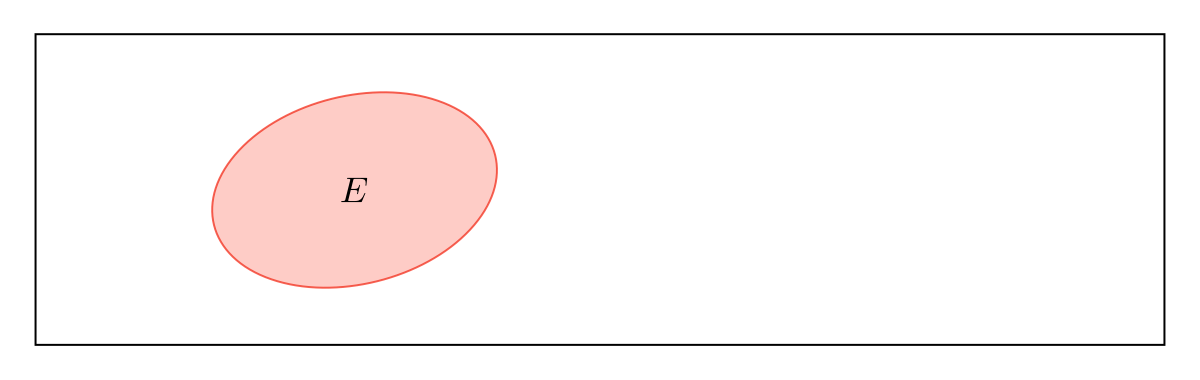
\includegraphics[width = 0.8\textwidth]{figs/probability-axiom-1.png}
\end{figure}

\item \textbf{Axioma de la certeza}: 
$$P(S) = 1$$
La probabilidad del espacio muestral $S$ es igual a 1. Esto significa que la probabilidad de que ocurra algún evento en el espacio muestral es 100\%.
\begin{figure}[h]
\centering
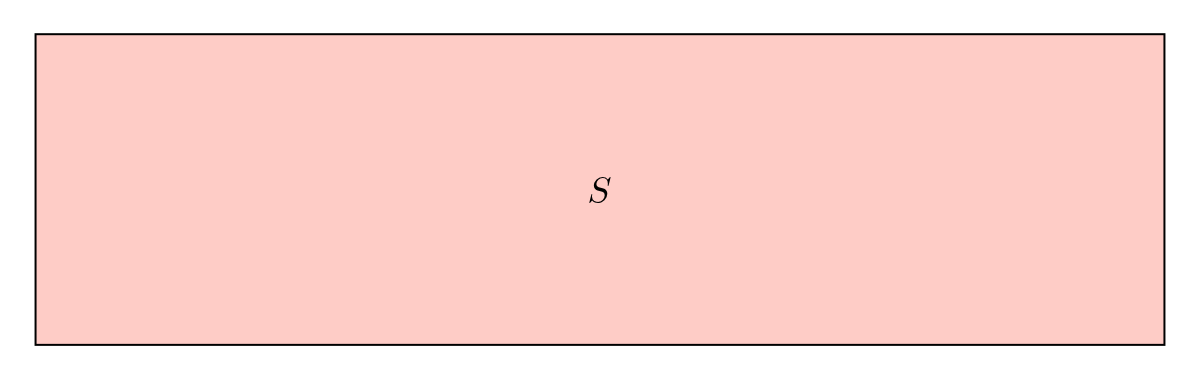
\includegraphics[width = 0.8\textwidth]{figs/probability-axiom-2.png}
\end{figure}

\item \textbf{Axioma de aditividad}: 
$$P\left(\bigcup_{i=1}^{n} A_i\right) = \sum_{i=1}^{n} P(A_i)$$
Para cualquier secuencia de eventos mutuamente excluyentes $[A_1,A_2,…,A_n]$, la probabilidad de la unión de estos eventos ($A_i$) es igual a la suma de las probabilidades de cada evento individual. Esto es que, si varios eventos que no pueden ocurrir simultáneamente, la probabilidad de que ocurra al menos uno de ellos es la suma de las probabilidades de cada uno de esos eventos.
\begin{figure}[h]
\centering
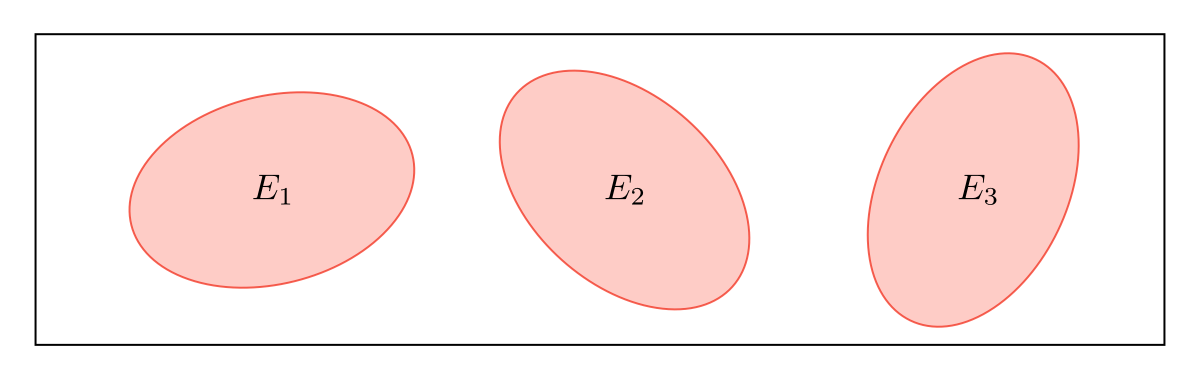
\includegraphics[width = 0.8\textwidth]{figs/probability-axiom-3.png}
\end{figure}
Teniendo en cuenta que $P(A_i) \leq P(S) = \sum_{i=1}^{n} P(A_i) = 1$, entonces: $0 \leq P(A) \leq 1$  para un evento $A_i$.

\end{enumerate}

\subsubsection{Combinatoria}
\begin{enumerate}
\item \textbf{Permutación}: es una disposición de $r$ objetos de un conjunto de $n$ objetos, **en un orden específico**. En otras palabras, es una forma de organizar o reordenar los elementos de un conjunto. Por ejemplo, si tienes un conjunto de tres letras: A, B y C, las posibles permutaciones de estas letras serían: [ABC, ACB, BAC, BCA, CAB, CBA].
La fórmula para calcular el número de permutaciones se da por: 
$$P(n, r) = \frac{n!}{(n-r)!}$$ 
donde:
\begin{itemize}
\item $P(n, r)$ es el número de permutaciones.
\item $n$ es el número total de objetos en el conjunto.
\item $r$ es el número de objetos que se seleccionan.
\item $n!$ (factorial de $n$) es el producto de todos los números enteros positivos hasta $n$.
\end{itemize}

Por ejemplo, si tienes un conjunto de 5 objetos y quieres seleccionar 3 de ellos en un orden específico, el número de permutaciones sería: $P(5, 3) = \frac{5!}{(5-3)!} = \frac{5!}{2!} = \frac{5 \times 4 \times 3 \times 2 \times 1}{2 \times 1} = 60$

\item \textbf{Combinación}: Una combinación es una selección de $r$ objetos de un conjunto de $n$ objetos, donde el orden no importa. La fórmula para calcular el número de combinaciones se da por:
$$C(n, r) = \frac{n!}{n!(n-r)!}$$
donde:
\begin{itemize}
\item $C(n, r)$ es el número de permutaciones.
\item $n$ es el número total de objetos en el conjunto.
\item $r$ es el número de objetos que se seleccionan.
\item $n!$ (factorial de $n$) es el producto de todos los números enteros positivos hasta $n$.
\item $r!$ (factorial de $r$) es el producto de todos los números enteros positivos hasta $r$.
\end{itemize}

Por ejemplo, si tienes un conjunto de 4 nucleótidos (A, T, C, G) y quieres seleccionar 3 de ellos sin importar el orden, el número de combinaciones sería: $C(4, 3) = \frac{4!}{3!(4-3)!} = \frac{4 \times 3 \times 2 \times 1}{3 \times 2 \times 1 \times 1} = 4$. Esto significa que hay 4 combinaciones posibles de 3 nucleótidos a partir de un conjunto de 4 nucleótidos.

\end{enumerate}

\subsection{Probabilidad condicional}
\subsubsection{Regla de Bayes}
Para eventos A y B, tal que $P(B)>0$:
$$P(A \mid B)=\frac{P(B \mid A)P(A)}{P(B)}$$

\textbf{Nota}: $P(A \cap B) = P(A)P(B \mid A) = P(A \mid B)P(B)$.

\subsubsection{Partición}
Sea una colección de $n$ conjuntos $A_i$ donde cada conjunto no es vacío; expresado como $\{A_i, i \in [[1, n]]\}$ tal que para todo $i$, $A_i \neq \emptyset$. En otras palabras, cada conjunto $A_i$ contiene al menos un elemento. 

Verbosamente: \textit{Para una colección de $n$ conjuntos $A_i$, donde $i$ varía en un rango desde 1 hasta $n$ para cada uno de los conjuntos $A_i$ en la colección, se da la condición de que cada conjunto $A_i$ no es vacío.}

Decimos que $\{A_i\}$ es una partición si se cumplen las siguientes condiciones:
$$\text(i)\quad\forall i \neq j, A_i \cap A_j = \emptyset \quad \quad \text(ii)\quad \bigcup_{i=1}^{n} A_i = S$$
\begin{itemize}
\item \textbf{Mutuamente excluyentes}: Para todo $i \neq j$, $A\_i \cap A\_j = \emptyset$. Esto significa que los conjuntos $A_{i}$ y $A_{j}$ no tienen elementos en común.
\item \textbf{Cobertura completa}: La unión de todos los conjuntos $A\_i$ es igual al conjunto original $S$, es decir, $\bigcup_{i=1}^{n} A_i = S$.
\end{itemize}

En resumen, una partición de un conjunto $S$ es una colección de subconjuntos no vacíos, mutuamente excluyentes, cuya unión es el conjunto original $S$.

\begin{figure}[h]
\centering
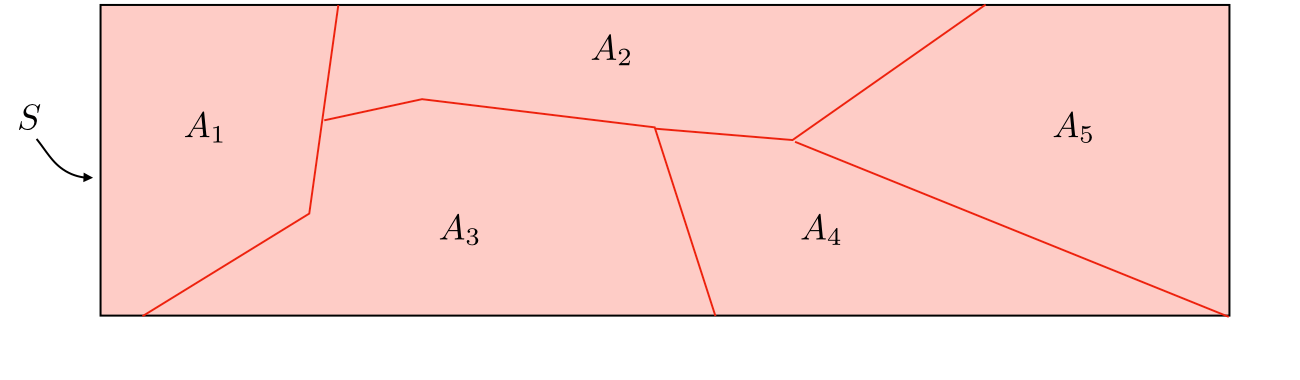
\includegraphics[width = 0.8\textwidth]{figs/partition.png}
\end{figure}

\subsubsection{Forma extendida de la regla de Bayes}
Esta fórmula nos permite calcular la probabilidad de un evento $A_k$ dado que ha ocurrido otro evento $B$, teniendo en cuenta todas las posibles particiones del espacio muestral.

La forma extendida de la regla de Bayes se utiliza cuando tenemos una partición del espacio muestral. Si $\\{A_{i}, i \in [[1, n]]}$ es una partición del espacio muestral, entonces la forma extendida de la regla de Bayes se expresa como:
$$P(A_k \mid B) = \frac{P(B \mid A_k) P(A_k)}{\sum_{i=1}^{n} P(B \mid A_i) P(A_i)}$$
donde:
\begin{itemize}
\item $P(A_{k} \mid B)$ es la probabilidad de que ocurra el evento $A_k$ dado que ha ocurrido el evento $B$.
\item $P(B \mid A_{k})$ es la probabilidad de que ocurra el evento $B$ dado que ha ocurrido el evento $A_k$.
\item $P(A_{k})$ es la probabilidad de que ocurra el evento $A_k$.
\item $\sum_{i=1}^{n} P(B \mid A_i) P(A_i)$ es la suma de las probabilidades de que ocurra el evento $B$ dado cada uno de los eventos $A_i$ multiplicadas por las probabilidades de que ocurra cada uno de los eventos $A_i$. Esta suma ponderada representa la probabilidad total de que ocurra el evento $B$, considerando todas las posibles particiones del espacio muestral.
\end{itemize}

\paragraph{Independencia}
Dos eventos $A$ y $B$ son independientes si y solo si la ocurrencia de uno no afecta la probabilidad de ocurrencia del otro.
$$P(A \cap B) = P(A)P(B)$$
Esto significa que la probabilidad de que ambos eventos ocurran simultáneamente es igual al producto de sus probabilidades individuales.

\subsection{Variables aleatorias}
\begin{figure}[h]
\centering
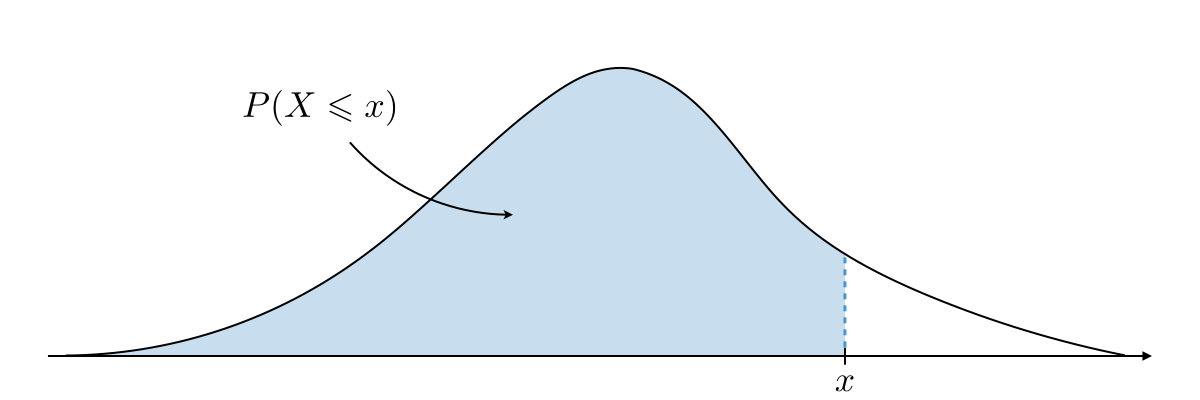
\includegraphics[width = 0.8\textwidth]{figs/cdf.png}
\end{figure}

%Esta parte de apuntes sobre probabilidad está actualmente en mantenimiento. Estamos trabajando arduamente para mejorar su experiencia. Por favor, vuelva a intentarlo más tarde.

